\chapter{Einführung}
Die rasanten Entwicklungen der Technologisierung und Digitalisierung haben branchenübergreifend einen Paradigmenwechsel eingeläutet. Die Konsequenz: Geräte wie beispielsweise Smartphones sind rund um die Uhr in sämtlichen Lebens- und Arbeitsbereichen aktiv, online und miteinander vernetzt. Digitale Geräte finden Einsatz im täglichen Leben und Arbeiten und so steht die Gesellschaft derzeit an der Schwelle zur vierten Industriellen Revolution.
%\fnurl{}{https://de.statista.com/statistik/daten/studie/309656/umfrage/prognose-zur-anzahl-der-smartphone-nutzer-weltweit/}

Damit einhergehend dringen neue Technologien, wie \textit{Virtual Reality} (VR) und \textit{Augmented Reality} (AR) in die globalen Märkte ein und beginnen die Entertainmentindustrie und die Arbeitswelt nachhaltig zu verändern. Durch die zunehmende Medienkompetenz und Offenheit der Gesellschaft ist die Bereitschaft vorhanden, neue Technologien zu nutzen. Es besteht daher ein hohes Interesse daran, geeignete Interaktionsmöglichkeiten für Aktionen im virtuellen Raum zu finden und zu erproben.
Das folgende Szenario verdeutlicht den Sachverhalt anhand einer Baumaschine und eines Maschinenführers im augmentierten Raum und stellt einen Rahmen für die prototypische Implementierung dar.
\paragraph*{Szenario der Anwendung}
Ein Maschinenführer befähigt eine Baumaschine mit Hilfe der Standard-Gesten der \textit{Microsoft HoloLens}, schwere reale Objekte von einer Position A zu Standort B zu befördern. Maschinen können heutzutage ohne weiteres Befehle von außen empfangen. Somit könnte der Maschinenführer die Maschine bequem und sicher in einer in 3D abstrahierten Replikation der Baustelle, die er in seiner Datenbrille sieht, bedienen. Er interagiert dann mit virtuellen Replikationen statt mit den echten Objekten auf der Baustelle. Die Interaktion mit den virtuellen Objekten wird über eine Netzwerkverbindung auf den Roboter übertragen, welcher dann das echte Objekt auf der realen Baustelle bewegt. Als Einsatzorte bieten sich menschenfeindliche Arbeitsumgebungen an, beispielsweise die Atmosphäre eines anderen Planeten, verseuchte oder unwegsame Gebiete der Erde oder das All.
In einer Arbeitsumgebung, in der nur Maschinen anwesend sind, kann kein Mensch zu Schaden kommen. Die Arbeiter wären keinen Witterungen oder gesundheitsgefährdenden Arbeitsumfeldern ausgesetzt. Resultat dessen wäre zwangsläufig weniger körperliche Erschöpfung, was wiederum weniger krankheitsbedingte Ausfälle der Maschinenführer bedeutet.
Die Interaktionsmöglichkeit mit den Maschinen wäre stets gegeben, so bleibt der menschliche Faktor, der alle Prozesse individuell der Situation anpassen kann, weiterhin gegeben und die Baustelle weiterhin wirtschaftlich.
\paragraph*{Fragestellung}
Aus diesem Szenario resultieren verschiedene Fragestellungen. Allen voran die Frage danach, wie der Mensch \frqq Herr der Maschinen\flqq\ bleiben kann. Welche Technologien eignen sich dazu, die Maschinenprozesse zu überwachen und zu beobachten? Und welche Interaktionen eignen sich am besten, einer Maschine Befehle zu erteilen, sowohl als Teleoperator als auch in enger räumlicher Zusammenarbeit mit der Maschine?

Um diese Fragen beantworten zu können, werden im Rahmen der vorliegenden Arbeit ein Konzept und eine prototypische Implementierung einer Industriemaschine im virtuellen Raum erstellt. Die Applikation wird mit innovativen Interaktionen bestückt und die Anwendung im Kontext der Industrie 4.0 diskutiert.

\section{Motivation und Kurzbeschreibung}
Innovative Ideen, Konzepte und Produkte zeichnen die Informatik und IT-Branche aus wie keine andere. So gilt es stets, neue Technologien zu erforschen, zu erlernen und frühzeitig Anwendungen und Konzepte auszuarbeiten, welche die Gesellschaft nachhaltig verändern können. Fast kein Industriezweig bleibt unberührt von diesen neuartigen, agilen Methoden und Konzepten. Datenbrillen, seien es nun VR oder AR \textit{Head-Mounted Display} (HMD) sind in ihrer \textit{Consumerversion} beziehungsweise als \textit{Development-Kit} auf den Märkten verfügbar. Noch sind sie zwar teuer, allerdings haben erste Hersteller bereits Preissenkungen angekündigt. Steigende Verkaufszahlen deuten darauf hin, dass es der Traum vieler Menschen ist, eine Datenbrille zu besitzen, sei es zu Entertainmentzwecken oder, um Vorteile im Alltag und im Arbeitsleben zu genießen. Was im Comic-Band \frqq Batman of the Future\flqq\ noch futuristisch und utopisch klang, nämlich einen Roboter mit einer Datenbrille und Gesten fernzusteuern, ist heute Gegenstand zahlreicher Forschungen, wie auch dieser Arbeit. In einer Episode des Bandes benutzt einer der Akteure einen riesigen Roboter als Baumaschine. Er steuert ihn über eine Datenbrille und Gesten, wie in Abbildung \ref{fig:BotF_Datenbrille} zu sehen.\begin{figure}[ht]
	\centering
	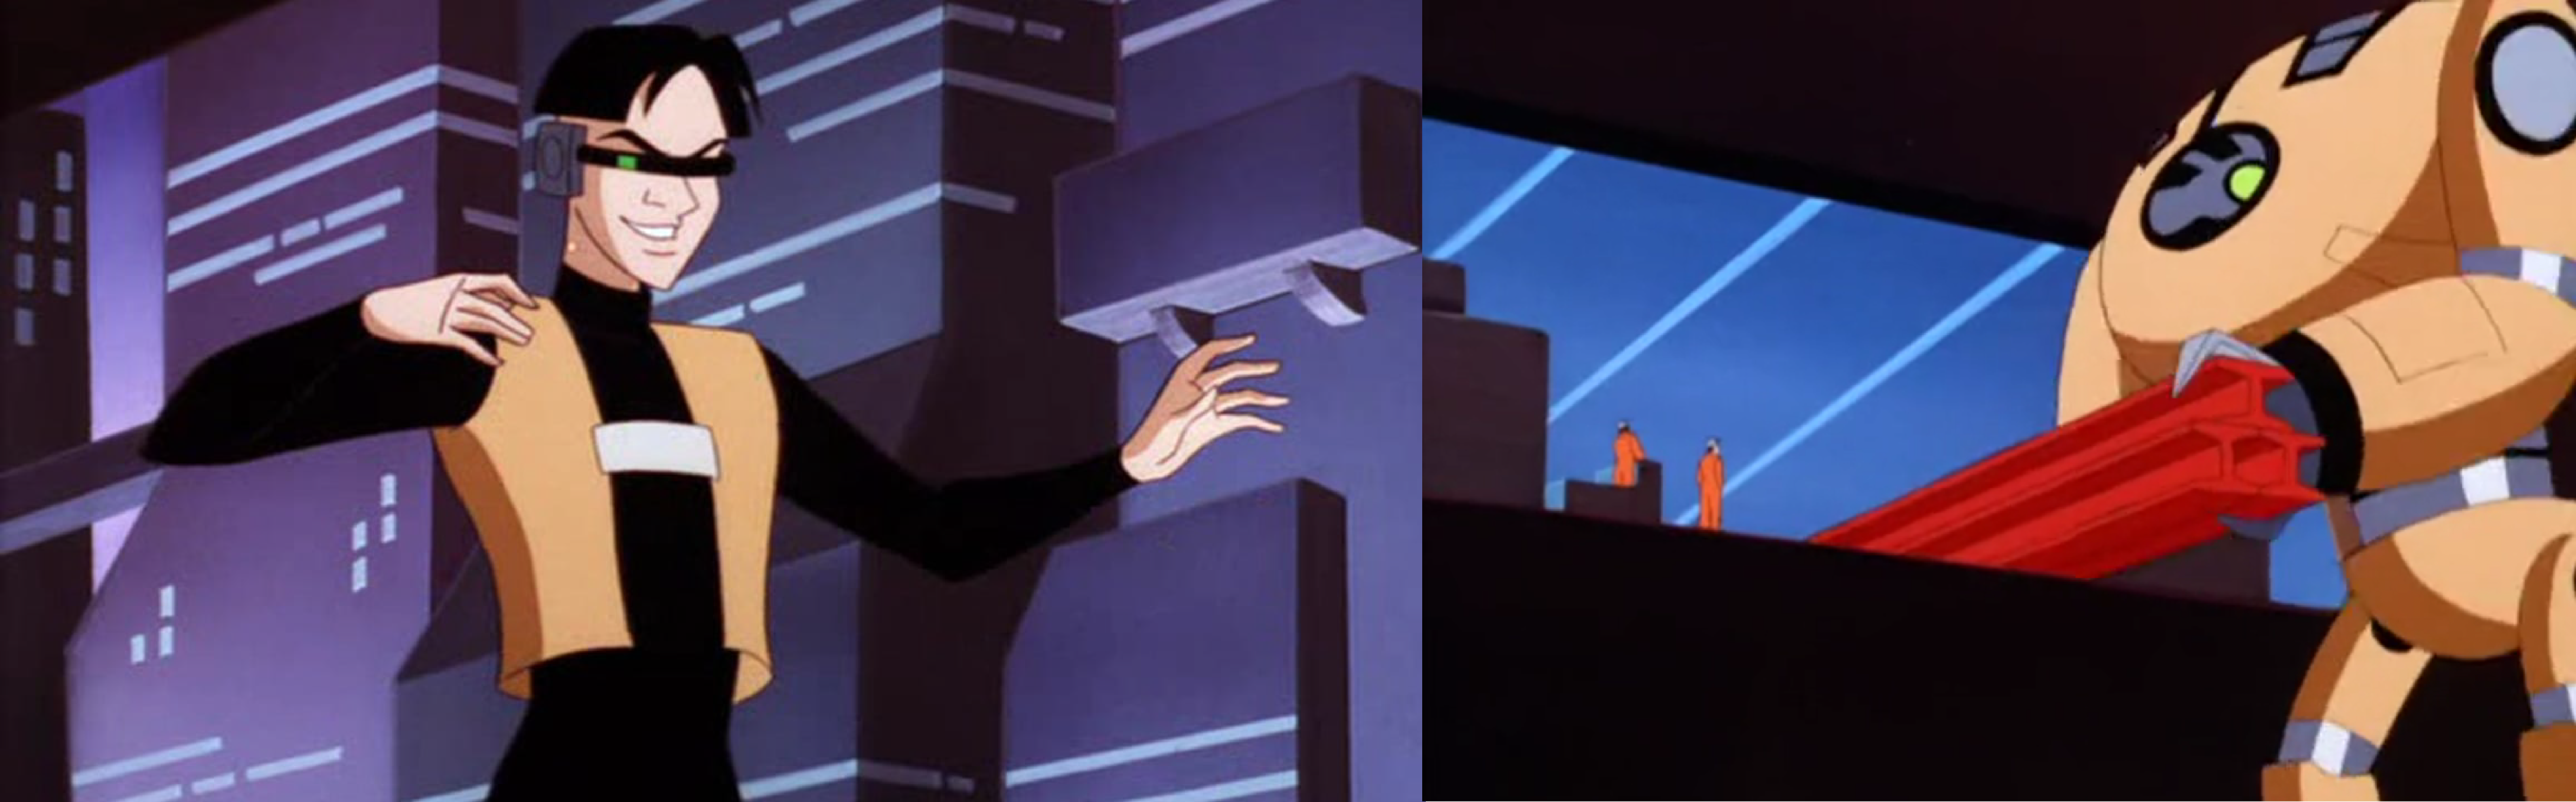
\includegraphics[width=.75\textwidth]{figuren/billy}
	\caption{Datenbrille in \frqq Batman of the Future\flqq. Bildquelle: \cite{billy}.}
	\label{fig:BotF_Datenbrille}
\end{figure} Um die Gesellschaft auf künftige Technologien vorzubereiten bedarf es Anwendungen, die diese Neuerungen erforschen, in ansehnlichen Szenarien darstellen und mit gutem Design und vorausschauenden Konzepten die Berührungsängste mit ihnen minimieren.

%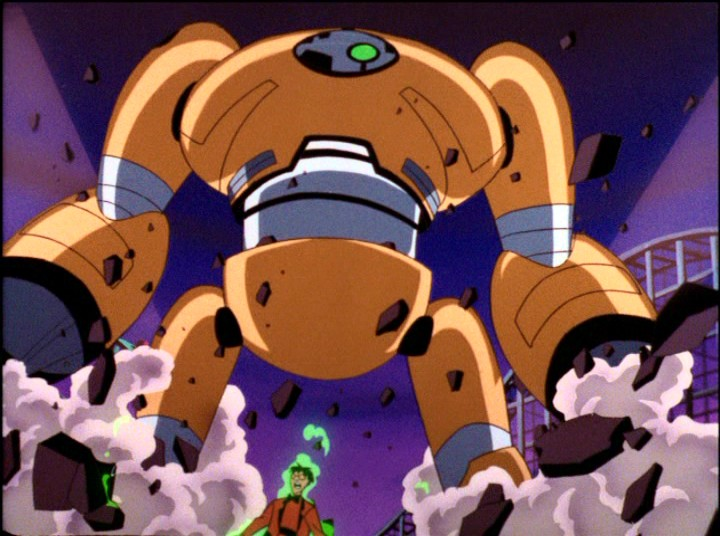
\includegraphics[width=1.0\textwidth]{figuren/golem}\vspace{1cm}
\section{Aufbau}
Ziel der vorliegenden Arbeit soll es sein, mit Hilfe eines Prototyps einen Ausblick darauf zu geben, wie Menschen in Zukunft mit Maschinen interagieren, was dabei zu beachten ist und welche Interaktionsformen sich für industrielle Zwecke besonders eignen. Im Anschluss an eine ausführliche Definition der grundlegenden Begrifflichkeiten im Kapitel~\ref{chapter:Grundlagen} erfolgt eine Analyse des aktuellen Forschungsstandes sowie eine Erörterung der Plausibilität der Fragestellung dieser Arbeit. Unter anderem wird in diesem Zuge auch erläutert, weshalb \textit{Microsofts HoloLens} und \textit{Legos EV3} geeignete Geräte für die prototypische Implementierung sind. Im Anschluss werden die Relevanz und die Potentiale der Technologien Robotik, Datenbrillen und AR für Forschungseinrichtungen, Industrieunternehmen und Technik-Enthusiasten erläutert und außerdem darauf eingegangen, inwieweit die \frqq Industrie 4.0\flqq\ als ganzheitliches Konzept dahinter steht. 

Danach wird in Kapitel~\ref{chapter:Konzeption} ein Konzept erarbeitet und präsentiert, welches sich damit auseinandersetzt, wie über eine Datenbrille in Form einer \textit{Microsoft HoloLens} eine Maschine, im prototypischen Fall ein Roboter aus \textit{Lego}, gesteuert und bei seiner Arbeit mit einem \textit{User Interface} augmentiert wird. Besagtes Vorhaben gilt es in Kapiel~\ref{chap:appImplementation} in einer Anwendung minimalisiert darzustellen und einen konzeptionellen Beweis dafür zu liefern, dass Interaktionen im virtuellen Raum auf die reale Welt übertragen werden können, einen Mehrwert bedeuten und dass sie im Kontext der vierten Industriellen Revolution eine Berechtigung besitzen. Abschließend wird diese These in Kapitel~\ref{chapter:UsabilityTest} mit einer benutzerbasierten, qualitativen Evaluation, dem \textit{Thinking-Aloud} Test, überprüft und dessen Ergebnisse ausgewertet.